\documentclass[11pt]{report}
\usepackage[spanish]{babel}
\decimalpoint
\usepackage[utf8]{inputenc}
\usepackage{amsmath}
\usepackage{listings}
\usepackage[usenames]{color} %seteamos el uso de nombre y color
\definecolor{gray97}{gray}{.97}%definimos nombre y color
\usepackage{textcomp}
\lstset{
	frame=Ltb,
	framerule=1pt,
	framextopmargin=5pt, %margen de arriba
	framexbottommargin=5pt, %margen de abajo
	framexleftmargin= 2pt, %separacion del margen izquierdo
	framesep=5pt,
	rulesep=0.3pt,
	backgroundcolor=\color{gray97},
	rulesepcolor=,
	tabsize=2,
	rulecolor=\color[RGB]{106, 182, 217}, %AZUL
	upquote=true,
	aboveskip={2\baselineskip}, %despues de la linea de texto
	columns=fixed,
	showstringspaces=false,
	extendedchars=true,
	breaklines=true,
	prebreak = \raisebox{0ex}[0ex][0ex]{\ensuremath{\hookleftarrow}},
	showtabs=false,
	showspaces=false,
	showstringspaces=false,
	basicstyle=\scriptsize\ttfamily\color[RGB]{39, 100, 46}, %Numeros de lineas, simbolos, puntos y coma y demas
	identifierstyle=\ttfamily\color[RGB]{56, 140, 189}, %variables
	commentstyle=\color[RGB]{62, 179, 101}, %comentarios
	stringstyle=\color[RGB]{247, 165, 42}, %impresiones
	keywordstyle=\bfseries\color[RGB]{237, 118, 150}, %funciones
	%
	numbers=left,
	numbersep=1pt, %separacion del numero
	numberstyle=\tiny,
	numberfirstline = false,
	breaklines=true,
}
\usepackage{textcomp}
\usepackage{graphicx}
\usepackage[colorinlistoftodos]{todonotes}
\usepackage{eso-pic}
\usepackage{avant}
\usepackage[top=1.8cm,bottom=1.8cm,left=2cm,right=2cm,headsep=8pt,a4paper]{geometry}
\usepackage{fancyhdr}
\pagestyle{fancy}
\fancyhf{}
%\fancyhead[LE,RO]{UNSAAC 2019-II}
%\fancyhead[RE,LO]{Ingenieria Electrónica}
%\fancyfoot[CE,CO]{\leftmark}
\fancyfoot[CO]{\thepage}
\renewcommand{\headrulewidth}{1pt}
\renewcommand{\footrulewidth}{1pt}
\usepackage{tabu}
\usepackage{array}
\usepackage{multirow}
\usepackage{amssymb}
\usepackage{makeidx}
\usepackage{wrapfig}
\usepackage{enumerate}
\usepackage{amsmath,tikz}
\usepackage{steinmetz}
\newcommand*{\horzbar}{\rule[0.05ex]{2.5ex}{0.5pt}}
\usepackage{calc}
\usepackage{dsfont}
\usepackage{enumitem}
\usepackage{subfig}

\title{
	\textsc{Universidad Nacional de San Antonio Abad del Cusco}\\
	\textbf{Compuertas Lógicas}\\
	Preinforme 1}

\author{
	\begin{tabular}{lr}
		Edison \textsc{Abado Ancco} & 145012 \\
		Roly Sandro \textsc{Gutierrez Benito} & 182967\\
	\end{tabular}
}


\begin{document}
	
\begin{titlepage}
	\newcommand{\HRule}{\rule{\linewidth}{0.5mm}} 
	\center
	\textsc{\LARGE  Universidad Nacional de San \\[0.2cm] Antonio Abad del Cusco}\\[1.5cm] 
	
\includegraphics[width=4cm]{IMAGENES/escudo}\\[1cm]
	\textsc{\Large Facultad de Ingeniería Eléctrica, \\ Electrónica, Informática y Mecánica}\\[0.5cm] 
	\textsc{\large Escuela Profesional de Ingeniería Electrónica}\\[0.5cm]
	\textsc{\Large \textbf{Antenas}}\\[0.5cm] 
	\HRule \\[0.4cm]
	{ \huge \bfseries Distribuciones de Corriente}\\[0.4cm] 
	\HRule \\[1.5cm]
	\begin{minipage}{\textwidth}
		\center 
		
		\emph{Profesor:} \\
		Ing. Milton \textsc{Velasquez Curo} \\[1cm]
		
		\begin{tabular}{c}
			\emph{Alumnos:}  \\
			Edison   \textsc{Abado Ancco} \\
			Roly Sandro    \textsc{Gutierrez Benito} \\
			Jhon Saul   \textsc{Huallpa Aimituma} \\
			Anel Milenka   \textsc{Delgado Cama} \\
			Ronny  \textsc{Vilavila Contreras} \\
			Maria Fernanda    \textsc{Pilares Aguirre} \\
			Luis Angel  \textsc{Mendoza Saya} \\
		\end{tabular}
	\end{minipage}\\[2cm]
	\today
\end{titlepage}


\newpage

%\tableofcontents indice bloqueado xD

\chapter{Distribuciones de corrientes para una agrupación lineal de N elementos}

Para todas las distribuciones usamos los de cada parámetro de acuerdo a la imagen \eqref{img1}.



\begin{figure}[h!]
	\centering
	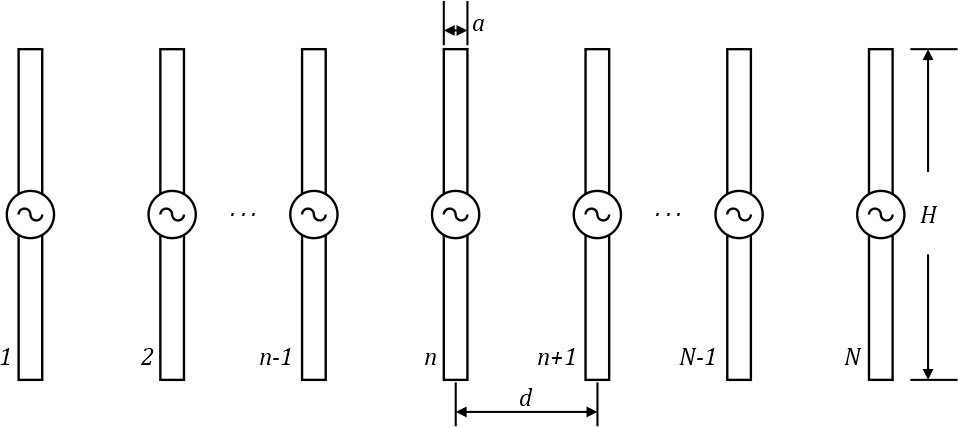
\includegraphics[scale=1]{IMAGENES/img1}
	\caption{Definición de variables.}
	\label{img1} % Debe estar al final del contenido de la figura
\end{figure}

El parámetro $N$ es el único que se variará, donde $n$ es el elemento central; los siguientes parámetros son fijos.

\begin{align*}
	f =			& \ 300MHz \\
	\lambda = 	& \ 1.00m \\
	H =			& \ \lambda/2 = 0.5m \\
	a =			& \ 0.2mm \\
	d_1 = & \ \lambda / 2 = 0.5m \\
	d_2 = & \ \lambda / 4 = 0.25m \\
\end{align*}

Podemos determinar un aproximado de la directividad con:

\begin{equation}
	D = \frac{4\pi}{\int\int_{4/\pi} t(\theta,\phi)d\Omega}=\frac{4\pi}{\Omega_e}
\end{equation}

Donde $\Omega_e$ es el ángulo sólido, definido como el ángulo dado a $-3dB$ en el patrón de radiación, y se usará para hacer comparaciones. De la teoría podemos considerar que las antenas directivas, con un sólo lóbulo principal y lóbulos secundarios de valores reducidos, podemos tener una estimación de la directividad considerando que se produce radiación uniforme en el ángulo sólido definido por los anchos de haz a $-3dB$ en los dos planos principales del patron de radiación ($\Omega_e = \Delta\theta_1 \cdot \Delta\theta_2$)

\section{Comparación para 3, 5, 7 y 9 elementos}

A continuación se hacen las comparaciones de patrones de radiación de corte horizontal y vertical. Las ganancias máximas entre el corte horizontal y vertical son prácticamente la misma para una determinada configuración de elementos.

\newpage

\subsection{Comparación de distribuciones para 3 elementos}

Las distribuciones de corrientes para 3 elementos están dados por:

\begin{tabular}{l|c|c|c}
	& $a_0$ & $a_1$ & $a_2$ \\ \hline
	Distribución Uniforme 	& 1 & 1 & 1  \\
	Distribución Triangular & 1 & 2 & 1  \\
	Distribución Binómica 	& 1 & 2 & 1  \\
\end{tabular}\\
 
Lo más resaltante es que las distribuciones Triangular y Binómica generan patrones de radiación superpuestas, ya que estos tienen los mismos valores de corriente para 3 elementos. 
La distribución de corriente que genera menor directividad es la Triangular, y las mayores son la uniforme junto a la binómica por estar superpuestas. 


% COMPARACIÓN PARA 3 ELEMENTOS
\begin{figure}[h!]
	\centering
	\subfloat[]{
		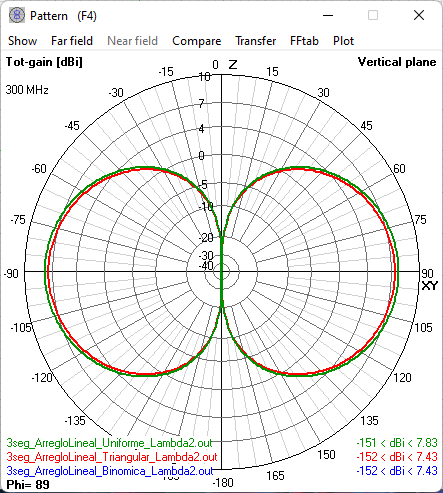
\includegraphics[scale=0.6]{IMAGENES/a131}\label{a131}}
	\subfloat[]{
		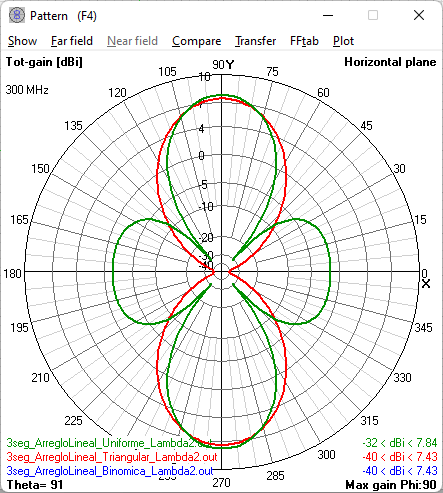
\includegraphics[scale=0.6]{IMAGENES/a132}\label{a132}}	\\
	\subfloat[]{
		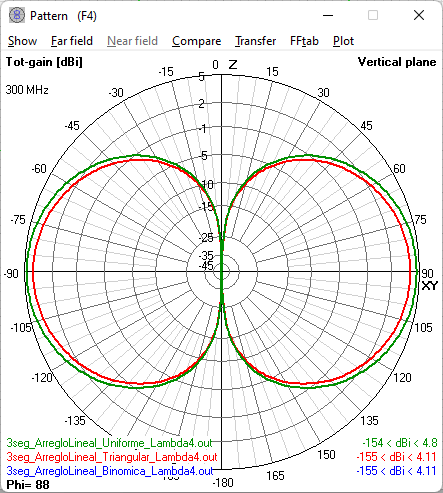
\includegraphics[scale=0.6]{IMAGENES/a133}\label{a133}}
	\subfloat[]{
		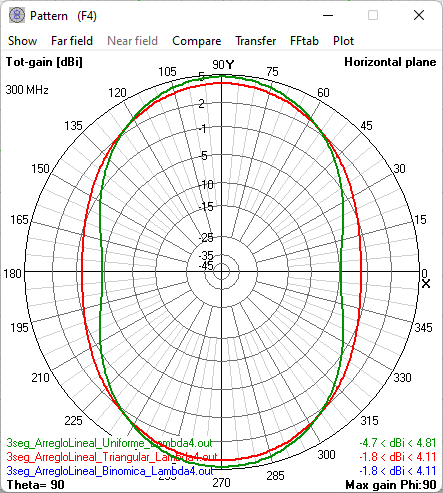
\includegraphics[scale=0.6]{IMAGENES/a134}\label{a134}}
	\caption{Patrones de radiación para 3 segmentos.
	(a) Vertical para $d =\lambda/2$.
	(b) Horizontal para $d=\lambda/2$.
	(c) Vertical para $d=\lambda/4$.
	(d) Horizontal para $d=\lambda/4$.}
\end{figure}


\subsection{Comparación de distribuciones para 5 elementos}

Las distribuciones de corrientes para 5 elementos están dados por: 

\begin{tabular}{l|c|c|c|c|c}
	& $a_0$ & $a_1$ & $a_2$ & $a_3$ & $a_4$\\ \hline
	Distribución Uniforme 	& 1 & 1 & 1 & 1 & 1 \\
	Distribución Triangular & 1 & 2 & 3 & 2 & 1 \\
	Distribución Binómica 	& 1 & 4 & 6 & 4 & 1 \\
\end{tabular} \\

La distribución triangular de obtiene de manera escalonada sumando $+1$ hasta el centro, y luego sumando $-1$ hasta el extremo opuesto. La distribución binómica se usa el triángulo de pascal para un $n = N - 1$ correspondiente. 
La distribución de corriente que genera menor directividad es la binómica, pero esta no presenta lóbulos secundarios, ya sea para $d_1$ o $d_2$; y la que mayor directividad presenta es la distribución uniforme, pero esta presenta dos o mas lobulos secundarios tanto para $d_1$ o $d_2$.


% COMPARACIÓN PARA 5 ELEMENTOS
\begin{figure}[h!]
	\centering
	\subfloat[]{
		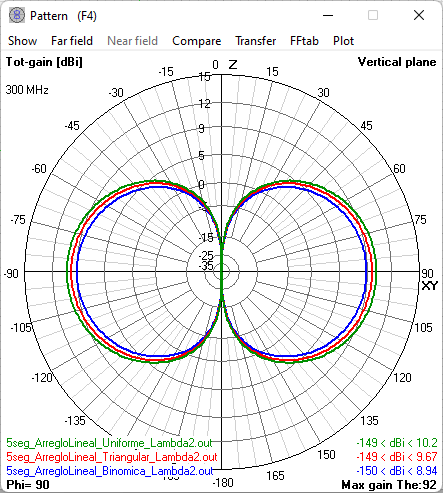
\includegraphics[scale=0.6]{IMAGENES/a151}\label{a151}}
	\subfloat[]{
		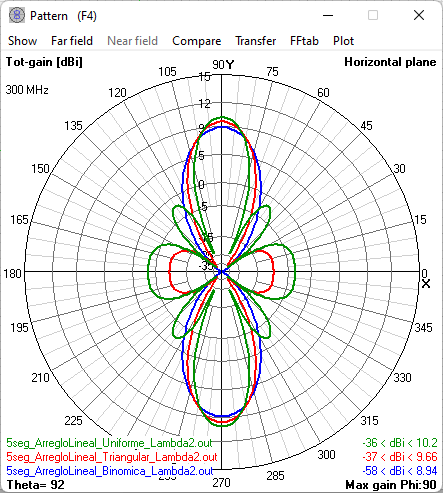
\includegraphics[scale=0.6]{IMAGENES/a152}\label{a152}}	\\
	\subfloat[]{
		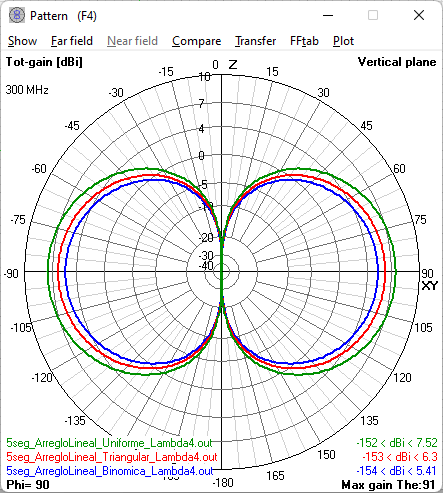
\includegraphics[scale=0.6]{IMAGENES/a153}\label{a153}}
	\subfloat[]{
		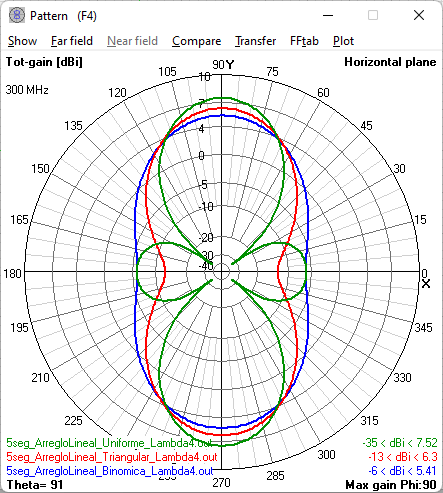
\includegraphics[scale=0.6]{IMAGENES/a154}\label{a154}}
	\caption{Patrones de radiación para 5 segmentos.
		(a) Vertical para $d_1 =\lambda/2$.
		(b) Horizontal para $d_1=\lambda/2$.
		(c) Vertical para $d_2=\lambda/4$.
		(d) Horizontal para $d_2=\lambda/4$.}
\end{figure}

\subsection{Comparación de distribuciones para 7 elementos}

Las distribuciones de corrientes para 7 elementos están dados por: 

\begin{tabular}{l|c|c|c|c|c|c|c}
	& $a_0$ & $a_1$ & $a_2$ & $a_3$ & $a_4$ & $a_5$ & $a_6$ \\ \hline
	Distribución Uniforme 	& 1 & 1 & 1 & 1 & 1 & 1 & 1 \\
	Distribución Triangular & 1 & 2 & 3 & 4 & 3 & 2 & 1 \\
	Distribución Binómica 	& 1 & 6 & 15 & 20 & 15 & 6 & 1 \\
\end{tabular} \\

La distribución triangular de obtiene de manera escalonada sumando $+1$ hasta el centro, y luego sumando $-1$ hasta el extremo opuesto. La distribución binómica se usa el triángulo de pascal para un $n = N - 1$ correspondiente. 
La distribución de corriente que genera menor directividad es la binómica, esta presenta lóbulos secundarios muy pequeños para $d_1$ y ninguna para $d_2$; la que mayor directividad presenta es la distribución triangular, pero es muy cercana a la distribución uniforme con la diferencia de que esta última presenta lóbulos secundarios laterales muy pronunciados para $d_1$; y la mayor directividad para $d_2$ la sigue teniendo la distribución uniforme.

% COMPARACIÓN PARA 7 ELEMENTOS
\begin{figure}[h!]
	\centering
	\subfloat[]{
		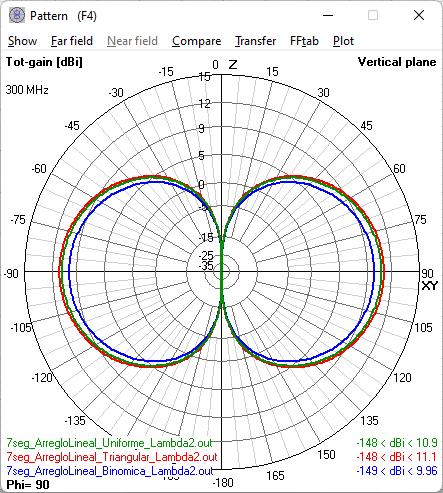
\includegraphics[scale=0.6]{IMAGENES/a171}\label{a171}}
	\subfloat[]{
		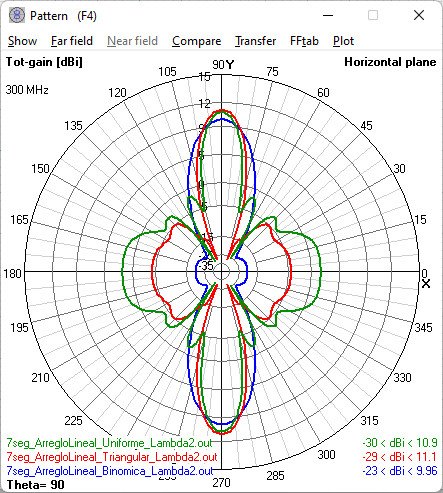
\includegraphics[scale=0.6]{IMAGENES/a172}\label{a172}}	\\
	\subfloat[]{
		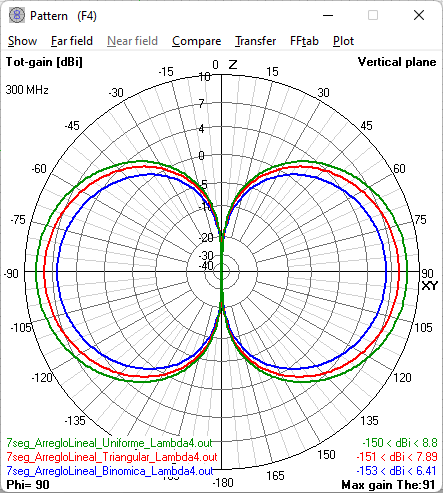
\includegraphics[scale=0.6]{IMAGENES/a173}\label{a173}}
	\subfloat[]{
		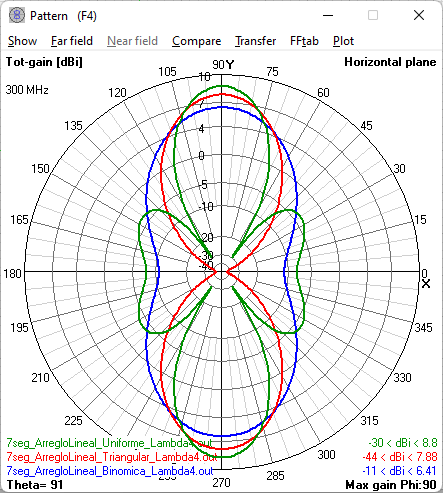
\includegraphics[scale=0.6]{IMAGENES/a174}\label{a174}}
	\caption{Patrones de radiación para 7 segmentos.
		(a) Vertical para $d_1 =\lambda/2$.
		(b) Horizontal para $d_1=\lambda/2$.
		(c) Vertical para $d_2=\lambda/4$.
		(d) Horizontal para $d_2=\lambda/4$.}
\end{figure}


\subsection{Comparación de distribuciones para 9 elementos}

Las distribuciones de corrientes para 9 elementos están dados por: 

\begin{tabular}{l|c|c|c|c|c|c|c|c|c}
	& $a_0$ & $a_1$ & $a_2$ & $a_3$ & $a_4$ & $a_5$ & $a_6$ & $a_7$ & $a_8$\\ \hline
	Distribución Uniforme 	& 1 & 1 & 1 & 1 & 1 & 1 & 1 & 1 & 1\\
	Distribución Triangular & 1 & 2 & 3 & 4 & 5 & 4 & 3 & 2 & 1\\
	Distribución Binómica 	& 1 & 8 & 28 & 56 & 70 & 56 & 28 & 8 & 1\\
\end{tabular} \\

La distribución triangular de obtiene de manera escalonada sumando $+1$ hasta el centro, y luego sumando $-1$ hasta el extremo opuesto. La distribución binómica se usa el triángulo de pascal para un $n = N - 1$ correspondiente. 
La distribución de corriente que genera menor directividad es la triangular para $d_1$, y la binómica para $d_2$; y la mayor directividad la presenta la distribución uniforme para $d_1$ y la distribución triangular para $d_2$.

% COMPARACIÓN PARA 9 ELEMENTOS
\begin{figure}[h!]
	\centering
	\subfloat[]{
		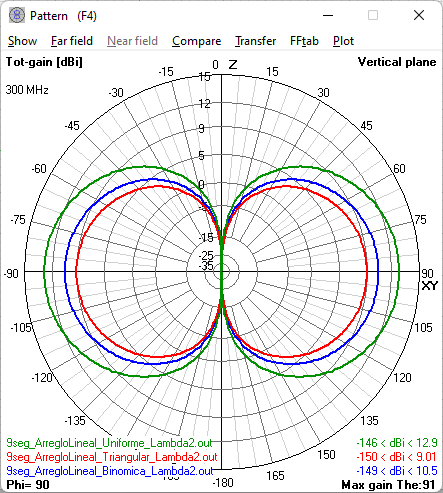
\includegraphics[scale=0.6]{IMAGENES/a191}\label{a191}}
	\subfloat[]{
		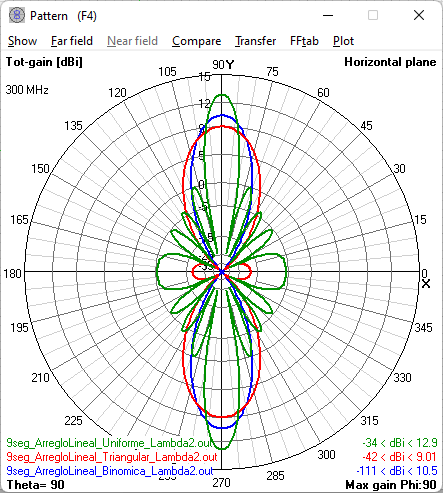
\includegraphics[scale=0.6]{IMAGENES/a192}\label{a192}}	\\
	\subfloat[]{
		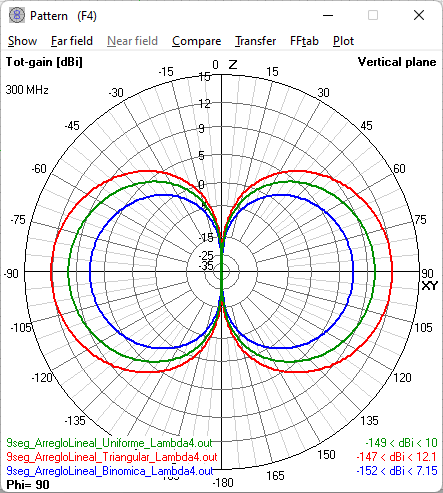
\includegraphics[scale=0.6]{IMAGENES/a193}\label{a193}}
	\subfloat[]{
		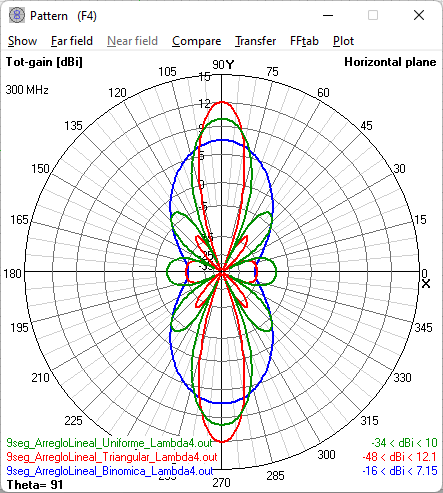
\includegraphics[scale=0.6]{IMAGENES/a194}\label{a194}}
	\caption{Patrones de radiación para 9 segmentos.
		(a) Vertical para $d_1 =\lambda/2$.
		(b) Horizontal para $d_1=\lambda/2$.
		(c) Vertical para $d_2=\lambda/4$.
		(d) Horizontal para $d_2=\lambda/4$.}
\end{figure}

\newpage

\section{Comparaciones para $d_1 = \lambda/2$ y $d_2 = \lambda/4$}

\subsection{Comparaciones para $\lambda$/2}

En estas comparaciones podemos ver que la distribución de corriente binómica es la que menos lóbulos secundarios y/o laterales presenta, por el otro lado se encuentra la distribución de corriente uniforme, que a medida que se le aumenta más elementos, su directividad aumenta, pero sus lóbulos secundarios aumentan en número, pero también se debe considerar que al aumentar número de lóbulos secundarios o menores, estos son pequeños. 

% COMPARACIÓN PARA d=LAMBDA/2
\begin{figure}[h!]
	\centering
	\subfloat[]{
		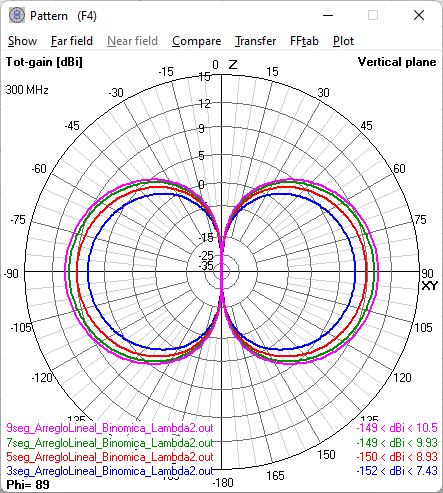
\includegraphics[scale=0.47]{IMAGENES/b11}\label{b11}}
	\subfloat[]{
		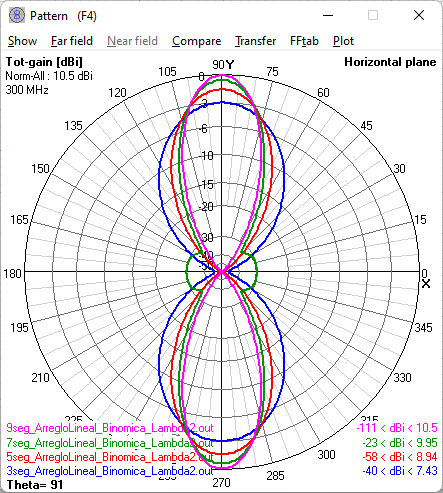
\includegraphics[scale=0.47]{IMAGENES/b12}\label{b12}}
	\subfloat[]{
		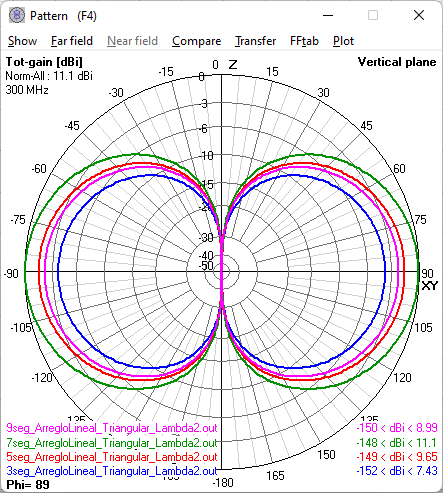
\includegraphics[scale=0.47]{IMAGENES/b13}\label{b13}}\\
	\subfloat[]{
		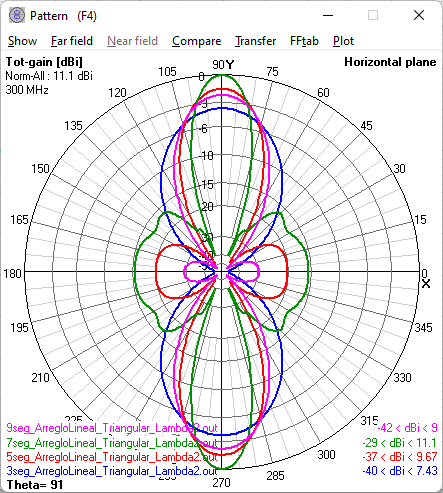
\includegraphics[scale=0.47]{IMAGENES/b14}\label{b14}}
	\subfloat[]{
		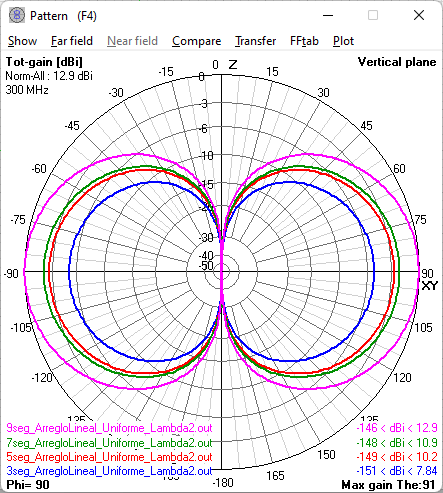
\includegraphics[scale=0.47]{IMAGENES/b15}\label{b15}}
	\subfloat[]{
		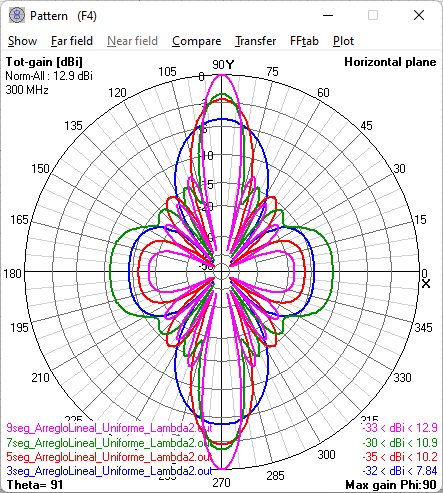
\includegraphics[scale=0.45]{IMAGENES/b16}\label{b16}}
	
	\caption{Patrones de radiación para $d_1=\lambda/2$.
		(a) Distribución Binómica Vertical.
		(b) Distribución Binómica Horizontal.
		(c) Distribución Triangular Vertical.
		(d) Distribución Triangular Horizontal.
		(e) Distribución Uniforme Vertical.
		(f) Distribución Uniforme Horizontal.}
\end{figure}

\newpage

\subsection{Comparaciones para $\lambda$/4}

En estas comparaciones podemos ver que la distribución de corriente binómica es la que ningún lóbulo secundarios y/o laterales presenta, por el otro lado se encuentra la distribución de corriente uniforme, que a medida que se le aumenta más elementos, su directividad aumenta, pero sus lóbulos secundarios aumentan en número, pero también se debe considerar que al aumentar número de lóbulos secundarios o menores, estos son pequeños. Debemos señalar que se alcanza una gran ganancia para la distribución triangular para 9 segmentos, se llega a $12.1dBi$ 

% COMPARACIÓN PARA d=LAMBDA/4
\begin{figure}[h!]
	\centering
	\subfloat[]{
		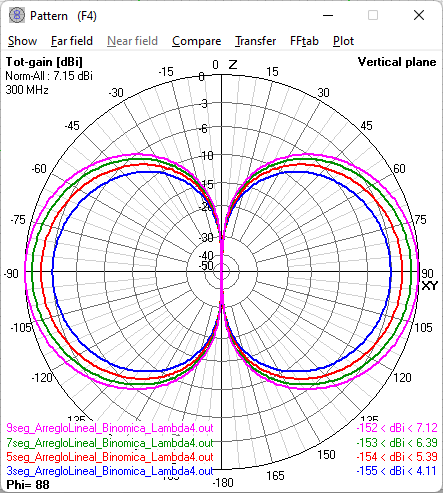
\includegraphics[scale=0.47]{IMAGENES/c11}\label{c11}}
	\subfloat[]{
		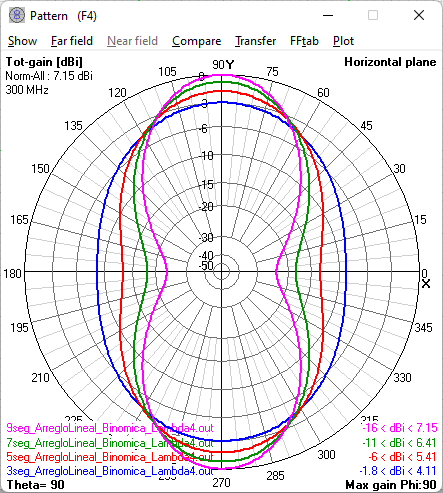
\includegraphics[scale=0.47]{IMAGENES/c12}\label{c12}}
	\subfloat[]{
		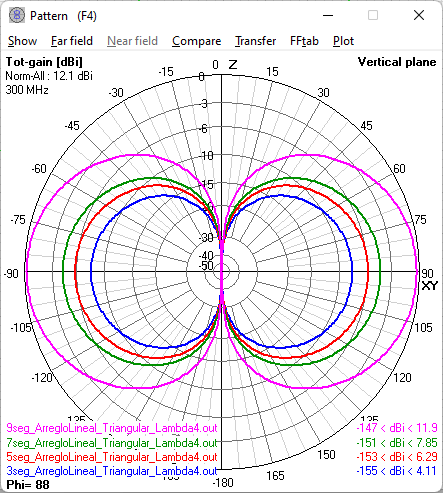
\includegraphics[scale=0.47]{IMAGENES/c13}\label{c13}}\\
	\subfloat[]{
		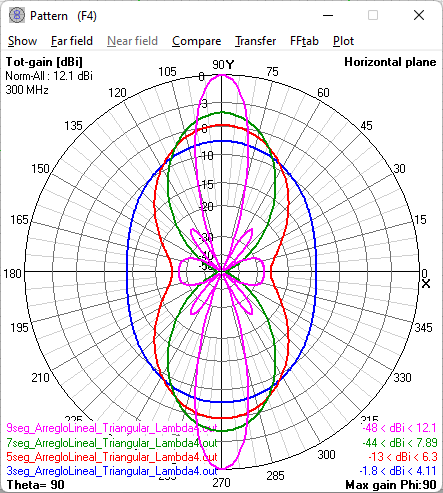
\includegraphics[scale=0.47]{IMAGENES/c14}\label{c14}}
	\subfloat[]{
		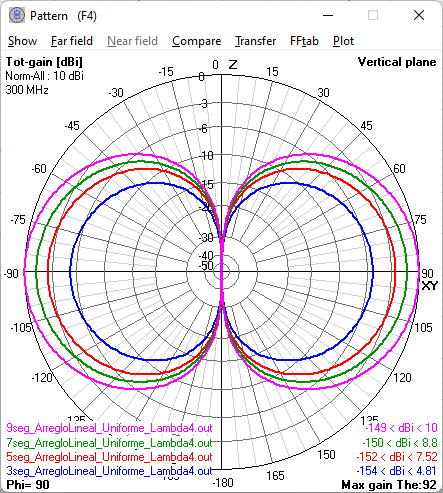
\includegraphics[scale=0.47]{IMAGENES/c15}\label{c15}}
	\subfloat[]{
		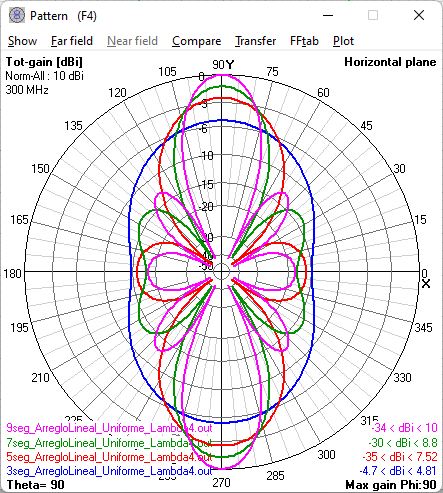
\includegraphics[scale=0.45]{IMAGENES/c16}\label{c16}}
	
	\caption{Patrones de radiación para $d_2=\lambda/4$.
		(a) Distribución Binómica Vertical.
		(b) Distribución Binómica Horizontal.
		(c) Distribución Triangular Vertical.
		(d) Distribución Triangular Horizontal.
		(e) Distribución Uniforme Vertical.
		(f) Distribución Uniforme Horizontal.}
\end{figure}

\newpage

\section{Conclusiones}

\begin{itemize}
	\item Por encima de todo, en cualquiera de las distribuciones, podemos afirmar que se obtiene mejor directividad, y por sonsiguiente mayor ganancia para $d_1=\lambda/2$, como se muestra en la imagen \eqref{comparacion}.
	\item Podemos mejorar la directividad y ganancia variando $H$ para ir considerando los valores de ROE y el coeficiente de reflexión en la frecuencia de resonancia por ejemplo.
	\item Entre los tres tipos de distribución, vemos que la mejor distribución es la uniforme, debido a que en principio se necesita menor potencia que las otras distribuciones, y la directividad va en aumento a medida de que se agregan más elementos. Además de que a menos número de elementos, $3$ o $5$ por ejemplo, es la que mayor ganancia tiene, y mejor directividad presenta.
\end{itemize}

\begin{figure}[h!]
	\centering
	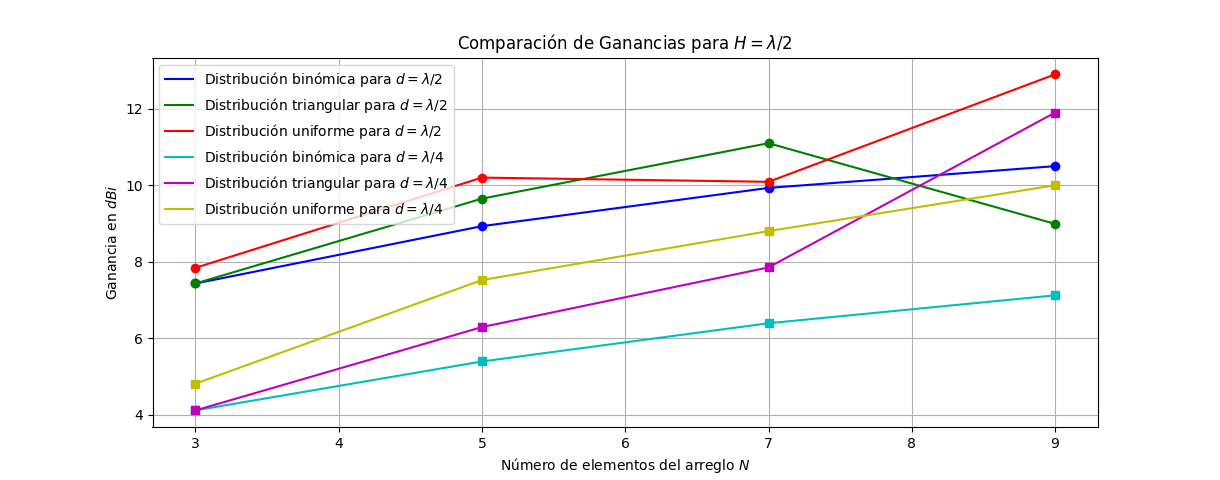
\includegraphics[scale=0.6]{IMAGENES/comparacion}
	\caption{Comparación de las ganancias para cada caso.}
	\label{comparacion}
\end{figure}


	
\end{document}
